% B1 figure caption (IEEE/RAL — paste below 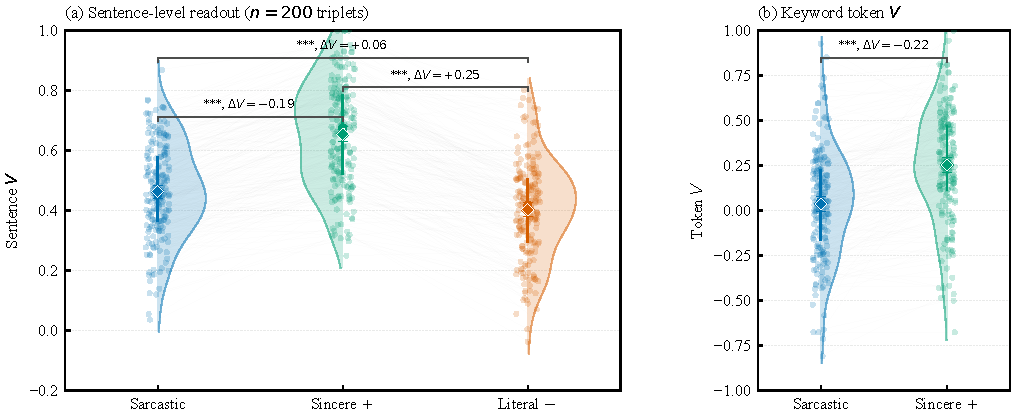
\includegraphics{b1_valence_raincloud.pdf})

\begin{figure*}[t]
  \centering
  \includegraphics[width=\textwidth]{figures/b1_valence_raincloud.pdf}
  \caption{Contextual sarcasm stress test ($n{=}200$ triplets, Qwen2.5-0.5B, E1 en/pole\_50 scaler).
  \textbf{(a)} Sentence-level projected valence $V$ for sarcastic (S), sincere-positive (P), and literal-negative (N) utterances after manual contextual rewrite.
  Rainclouds show kernel density (half-violin), IQR, jittered per-triplet scores, and bootstrap mean $\pm$95\% CI (diamonds); faint lines connect matched triplets.
  S and N largely co-locate (81.5\% $|V_S-V_N|<0.15$); Wilcoxon signed-rank, paired $n{=}200$.
  \textbf{(b)} Token-level $V$ at the primary anchored positive keyword in S vs.\ P ($n{=}194$ hits); mean $\Delta V_{S-P}=-0.22$.}
  \label{fig:b1_sarcasm_raincloud}
\end{figure*}
